% !TEX root = base.tex 


\chapter{Experimental Overview}
\label{ch:experimental}


\chintro{The purpose of this section is to provide an overview of the fabrication and
characterization methods presented in this document. The main methods of sample
fabrication covered in this chapter are solid state synthesis of polycrystalline ceramics
and pulsed laser deposition of thin films. Characterization methods include microscopy,
thin film phase and orientation characterization, and characterization of photochemical
activity.}


\section{Fabrication Methods}
\label{sec:exp.fabrication}


\subsection{Solid State Synthesis}
\label{subsec:exp.solidstate}


Ceramic pellets were fabricated for use as polycrystalline substrates for film deposition.
By using polycrystalline substrates, photochemical properties and film growth could be
examined as a function of substrate orientation. In many cases, film growth occurs
epitaxially across the entirety of a single substrate grain. The random texture of the
substrate allows for measurement of properties across all possible orientations. As
compared to growth on single crystals, where only low index orientations are typically
available, this provides a much more diverse set of orientation conditions for
examination. 

All polycrystalline substrates and deposition targets were fabricated using a conventional
solid state synthesis route. Starting powers of metal oxides or carbonates were measured
in the correct stoichiometric proportions for the desired ceramic phase. Specific powders
and purities are listed in the sintering recipes contained in Table
\ref{tab:sinteringrecipe}.
 
\begin{table} 

	\begin{center}
	\footnotesize
	\begin{tabular}{llrrrrrrrrr}


		\multicolumn{1}{c}{Material}&
		\multicolumn{2}{c}{Starting Powder} &  
		\multicolumn{2}{c}{Reaction Step} &  
		\multicolumn{2}{c}{Burnoff} &  
		\multicolumn{2}{c}{Densification} &  
		\multicolumn{2}{c}{Grain Growth}  \\	

		\cmidrule(lr){1-1}
		\cmidrule(lr){2-3}
		\cmidrule(lr){4-5}
		\cmidrule(lr){6-7}
		\cmidrule(lr){8-9}
		\cmidrule(lr){10-11}
		
   		\ce{Fe2O3} &
		\ce{Fe2O3} &
	 	99.945\% &
		\multicolumn{2}{c}{---} &
		\SI{600}{\degreeCelsius} &
		\SI{12}{\hour}  &
		\SI{1200}{\degreeCelsius} &
		\SI{12}{\hour}  &
		\multicolumn{2}{c}{---} \\[9pt]

   		\ce{SrTiO3} &
		\ce{SrTiO3} &
	 	99.97\% &
		\multicolumn{2}{c}{---} &
		\SI{900}{\degreeCelsius} &
		\SI{10}{\hour}  &
		\SI{1360}{\degreeCelsius} &
		\SI{10}{\hour}  &
		\SI{1470}{\degreeCelsius} &
		\SI{3}{\hour}\\[9pt]
				
%   		\ce{BaTiO3} &
%		\ce{BaTiO3} &
%	 	99.97\% &
%		\multicolumn{2}{c}{---} &
%		\SI{900}{\degreeCelsius} &
%		\SI{10}{\hour}  &
%		\SI{1230}{\degreeCelsius} &
%		\SI{10}{\hour}  &
%		\SI{1360}{\degreeCelsius} &
%		\SI{3}{\hour}\\[9pt]

   		\ce{BiFeO3} &
		\ce{Bi2O3} &
	 	99.99\% &
		\SI{650}{\degreeCelsius} &
		\SI{6}{\hour}  &
		\SI{600}{\degreeCelsius} &
		\SI{12}{\hour}  &
		\SI{750}{\degreeCelsius} &
		\SI{12}{\hour}  &
		\SI{850}{\degreeCelsius} &
		\SI{3}{\hour}\\
		
		&
		\ce{Fe2O3}&
		99.945\%&
		&
		&
		&
		&
		&
		&
		&
		\\
		
	\end{tabular}
	\end{center}
   	\caption[Sintering recipes for polycrystalline pellets]{%
   		Sintering recipes for polycrystalline pellets used in this work. All starting
powders were purchased from Alfa Aesar (Ward Hill, MA).}
   	\label{tab:sinteringrecipe}

\end{table}
These powders were ball milled in ethanol using yttria-stabilized zirconia (\abbr{YSZ})
grinding media (Inframet Advanced Materials, Manchester, \abbr{CT}). The powders were
typically ball milled overnight to ensure complete mixing of the starting powders. The
slurry was placed in a drying oven to drive off ethanol. The dry powders were placed in an
alumina crucible and calcined to promote reaction of the starting powders into the desired
final phase. After this reaction step, the powders were ball milled overnight in ethanol
again. Before ball milling, a small amount (typically 1-2~wt\%) of polyethylene glycol
(\abbr{PEG}, \abbr{MW}8000, ) was added to act as a binder.  After ball milling, the
powders were dried as before. % Add the company to PEG

Pellets were formed of the dried powders under uniaxial loads in a stainless steel die.
The diameter of the die was approximately \SI{1}{\centi\meter} for polycrystalline
substrates and \SI{2.5}{\centi\meter} for film growth targets. The sides of the die were
coated with a saturated solution of stearic acid in ethanol to act as a lubricant. A small
amount of powder was added to the die. The die was placed on a manual hydraulic press  and
subjected to a load of 5000~pounds. The applied load was immediately released, and the
pellet was ejected from the die. Pellets were placed in an alumina crucible, with a small
amount of excess powder forming a barrier between the crucible and the pellets. Additional
pellets were stacked, until the crucible was full or the desired number of pellets was
reached. Any excess powder was loosely poured on top of the pellets to reduce loss of
volatile elements to the atmosphere during sintering.

The crucible was placed in the furnace, and heated in air according to the desired
sintering program. The same furnace was used to fabricate all specimens in this work. The
furnace allows a programmable series of sintering steps. Typically, the furnace was held
first at a low temperature to burn off organic materials in the pellet. Next, the
temperature was increased to a point where densification and sintering occur. Finally, the
temperature was increased to promote grain growth. Depending on the material, one or more
of these steps may be omitted from the synthesis procedure.

After the samples were cooled to room temperature, they were removed from the crucible.
Substrates were lapped flat and polished to provide a high quality surface for film
growth, electron backscatter diffraction analysis, and photochemical reaction. All
polishing was done using an autopolisher (Logitech, \abbr{UK} Scotland). Samples were
affixed to glass substrates using melted wax (Logitech), which were held to a polishing
jig with a vacuum. Lapping was performed using a steel plate and \SI{9}{\micro\meter}
alumina slurry (Buehler, Lake Bluff, \abbr{IL}). Both sides of each sample were lapped
flat, ensuring that the sides were parallel and had a uniform flat surface. Deionized
water was used to remove lapping residue. After both sides were flat, one side was
polished. For final polishing,{ }\SI{0.01}{\micro\meter} colloidal silica (MasterMet 2,
Buehler) was used with a polyurethane plate. The slightly basic nature of the colloidal
silica results in a chemomechanical polishing process, ensuring a smooth, flat surface.
Polishing times varied for each material, but were on the order of \texttildelow30~minutes
for each sample. Each sample was examined using optical microscopy to verify the removal
of surface scratches and roughness. After polishing, the pellets were annealed a final
time to heal surface damage from polishing and thermally etch the grain boundaries. 


\subsection{Pulsed Laser Deposition}
\label{subsec:exp.pld}


Pulsed laser deposition (\abbr{PLD}) was used to fabricate the thin films discussed in
this document. Benefits of \abbr{PLD} benefits include the ability to deposit
stoichiometric oxides, rapid and simple changeout of target materials, precise control of
film thickness, and easy control of deposition conditions.\cite{Chrisey:1994ta} A pulsed
laser deposition system consists of a high power pulsed ultraviolet laser, a focusing
optic system, and a vacuum chamber including an optical window for the laser, a target
holder, and a substrate holder and heater. A schematic of the system used in this work is
presented in Figure \ref{fig:pldsetup}.
\begin{figure}[b]
	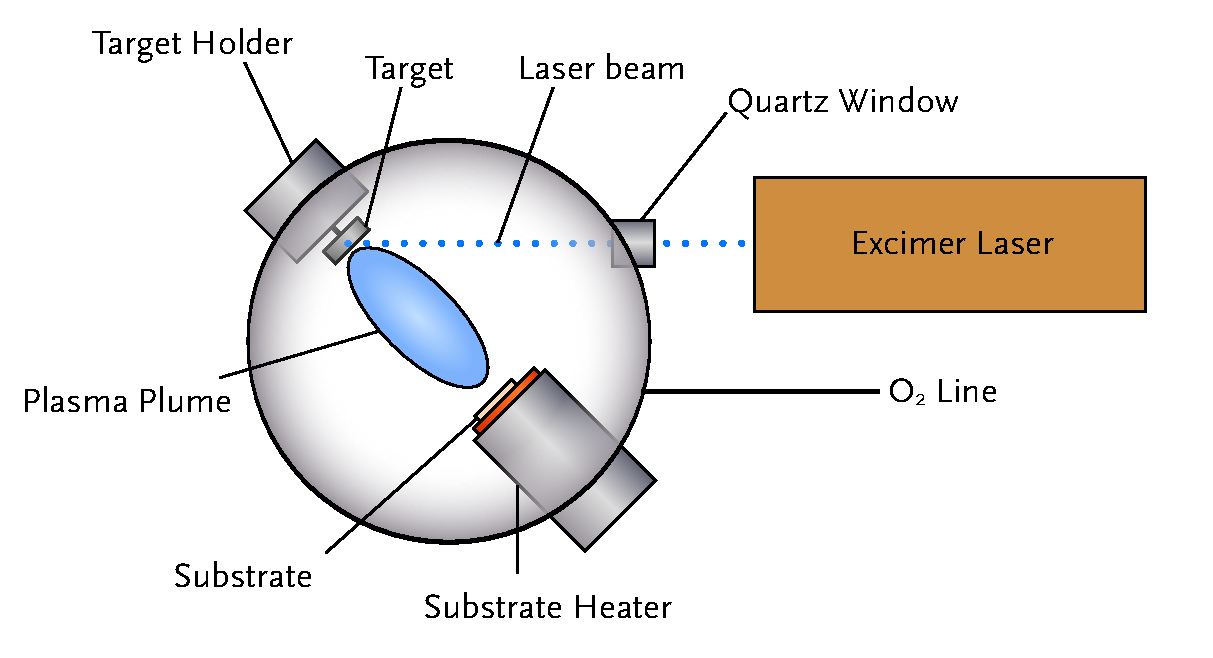
\includegraphics[width=\textwidth]{pldsetup.pdf}
	\caption[Schematic of pulsed laser deposition apparatus]{%
		Schematic of the pulsed laser deposition apparatus used in 
		this work, showing the location of the substrate and target, 
		and their relation to the pulsed laser beam.}
	\label{fig:pldsetup}
\end{figure}
The laser  beam enters the vacuum chamber through the quartz optical window. The beam is
aligned at a \SI{45}{\degree} angle from the target surface. The focused beam rapidly
heats the target material in a process called ablation. The high incident flux and energy
of the laser causes the formation of a plasma plume. The plume forms in a direction normal
to the surface of the target. The plume expands in the chamber, its shape and size
dependent on the energy of the laser pulse and the pressure of the process gas inside the
chamber. The substrate is affixed to a heater located parallel to the target material. As
the plume reaches the substrate, film nucleation and growth occurs. Each laser pulse
delivers a relatively consistent amount of film material to the substrate, and resulting
in typical growth rates on the order of \SI{0.01}{\nano\meter\per\pulse}. By determining
the growth rate via measurements of film thicknesses for films deposited with known
numbers of pulses, accurate values of film thicknesses can be obtained.

The key parameters controlled during pulsed laser deposition are the substrate
temperature, the pressure and composition of the process gas in the chamber, the
target-substrate distance, the laser energy, and the laser repetition rate. The substrate
temperature can strongly affect the crystallinity and phase of the resultant film. Higher
substrate temperature increases the crystallinity of the film, and increases the
likelihood of epitaxial growth.\cite{Francis:2004cf} The laser energy and repetition rate
combine to affect the rate of arrival of material to the substrate. At higher laser
energies, a greater amount of material is ablated from the target. If the laser repetition
rate is increased, the time between pulses is reduced, and the rate of ablated material
reaching the substrate is increased. By increasing or decreasing these values, kinetically
or thermodynamically stabilized film phases can be deposited. The substrate-target
distance affects the growth rate of the material. If the substrate is placed closer to the
target, a larger portion of the plasma plume is directed at the substrate, increasing the
growth rate. 

The process gas in the chamber during deposition and cooling affects film phase,
composition, and growth rate. A dynamic oxygen atmosphere is commonly used during
deposition to ensure the formation of oxide films. By varying the pressure of the oxygen
during deposition, various stoichiometric oxide compositions can be created from a single
metal or metal oxide target. Under high oxygen partial pressures, the formation of the
more highly oxidized material is favorable. The reverse is true under vacuum or low oxygen
pressures. In the scope of this work, a higher oxygen pressure during deposition creates
favorable conditions for the formation of the desired \ce{Fe2O3} phase rather than
\ce{FeO} or \ce{Fe3O4}. The atmosphere during post deposition annealing and cooling also
can affect the phase of the resulting film.

A commercially available pulsed laser deposition system from Neocera (Beltsville,
\abbr{MD}) was used for all film growth presented in this document. A KrF excimer laser
(Coherent, Santa Clara, \abbr{CA}) with a wavelength of \SI{248}{\nano\meter} was used for
ablation. Unless otherwise noted, substrates were cleaned ultrasonically in acetone and
then methanol. Substrates were affixed to the substrate heater with silver paint. The
substrate-target distance was fixed at \SI{6}{\centi\meter} for all depositions. The
chamber was evacuated to a base pressure of $10^{-5}$~\si{\torr} before substrate heating
began. Substrate heating and cooling rates were in the range of
20-30~\si{\degreeCelsius\per\minute}, as regulated by a programmable temperature
controller. While the substrate was heating, the target surface was cleaned by ablating it
with the laser. During target cleaning, a shield was kept in between the target and the
substrate to block the plume from reaching the substrate. Once deposition temperature was
reached, a dynamic oxygen atmosphere was established by flowing oxygen through the chamber
with the vacuum pump in operation. The shield between the target and substrate was
removed, and the target was hit with a predetermined number of laser pulses to deposit the
film. Immediately after deposition was completed, the chamber was sealed, and a static
oxygen atmosphere was introduced into the chamber while the substrate cooled. Growth
rates, laser energy, repetition rate, substrate temperature, and oxygen pressures were
controlled across all film depositions in this document. Table \ref{tab:pldparameters}
lists the values used. 
\begin{table} \small
\begin{center}
	\begin{tabular}{ll}

		Parameter &  
		Typical Value   \\
		
		\cmidrule(lr){1-1}
		\cmidrule(lr){2-2}
		
   		Substrate Temperature & 
		800~\si{\degreeCelsius} \\
		
  		Laser Energy & 
		160~\si{\milli\joule\per\pulse}  \\
		
		&
		(2~\si{\joule\per\centi\meter\squared}) \\
		
		Laser Rep Rate & 
		10~\si{\hertz} \\
		
		Deposition Gas Pressure & 
		200~\si{\milli\torr} \\
		
		Annealing Gas Pressure & 
		200~\si{\torr} \\
		
		Target Composition & 
		\textalpha-\ce{Fe2O3} \\
		
		Growth Rate & 
		0.01~\si{\nano\meter\per\second} \\

	\end{tabular}
	\end{center}
  	\caption[Experimental parameters for \ce{Fe2O3} film deposition]{%
		Experimental parameters for the deposition of \ce{Fe2O3} films. 
		These parameters were consistant across all depositions in this 
		document.}
	\label{tab:pldparameters}
\end{table}

The values used reflect conditions that produced the desired film results. Initial values
were selected based on typical values for users of this \abbr{PLD} chamber. Once films of
the desired phase were obtained, growth parameters were not further optimized. The only
variable altered from film to film was the numbers of pulses, which was varied to control
the resulting thickness of the deposited film.


\section{Characterization Methods}
\label{sec:exp.characterization}


\subsection{Marker Reactions}
\label{subsec:exp.markerreactions}

\begin{figure}
\begin{center}
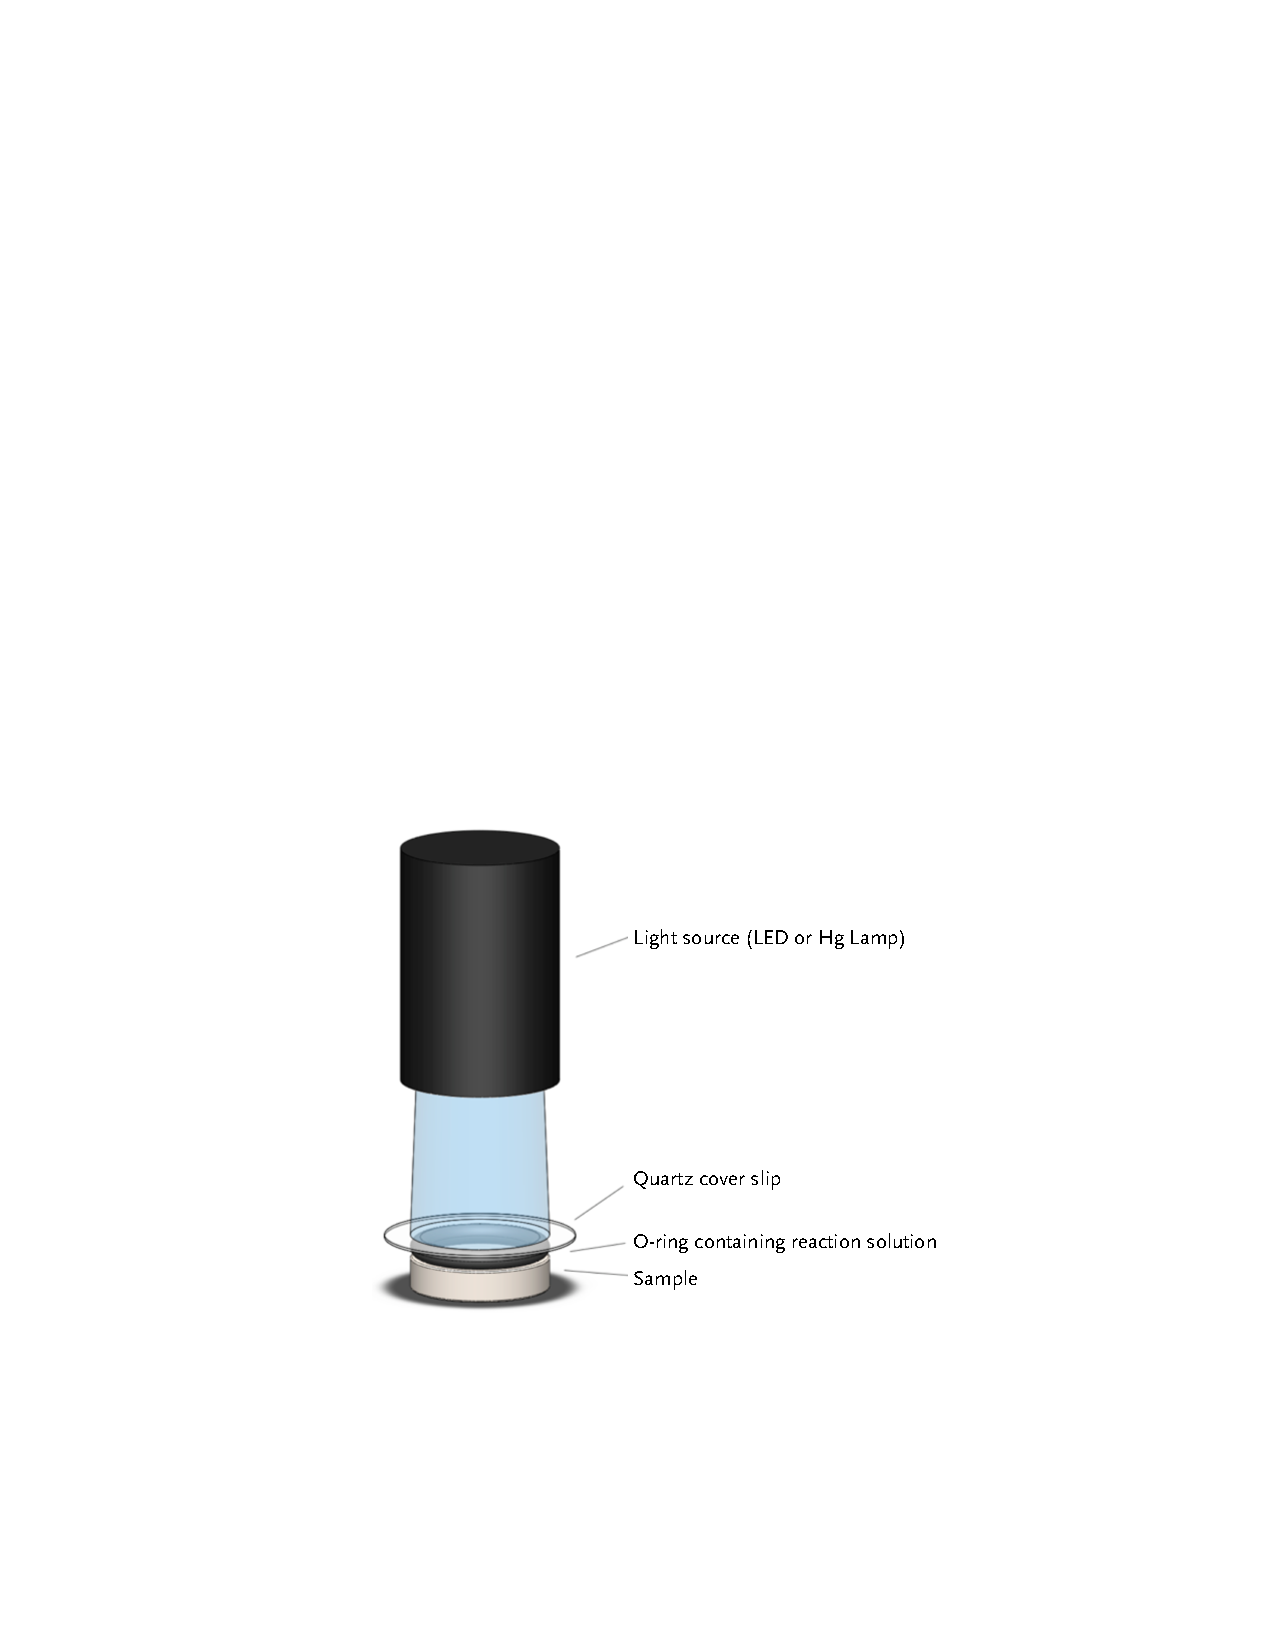
\includegraphics[width=0.8\textwidth]{rxnsetup.pdf}
\caption[Experimental setup for marker reactions]{%
	Experimental setup for performing photochemical marker 
	reactions. \ce{AgNO3} reaction solution is held in an 
	O-ring under a quartz cover slip and the light source 
	is positioned directly above the assembly.}
\label{fig:rxnsetup}
\end{center}
\end{figure}
%\sidefigure[Experimental setup for marker reactions]{%
%	Experimental setup for performing photochemical marker 
%	reactions. \ce{AgNO3} reaction solution is held in an 
%	O-ring under a quartz cover slip and the light source 
%	is positioned directly above the assembly.
%	\label{fig:rxnsetup}
%	}{%
%	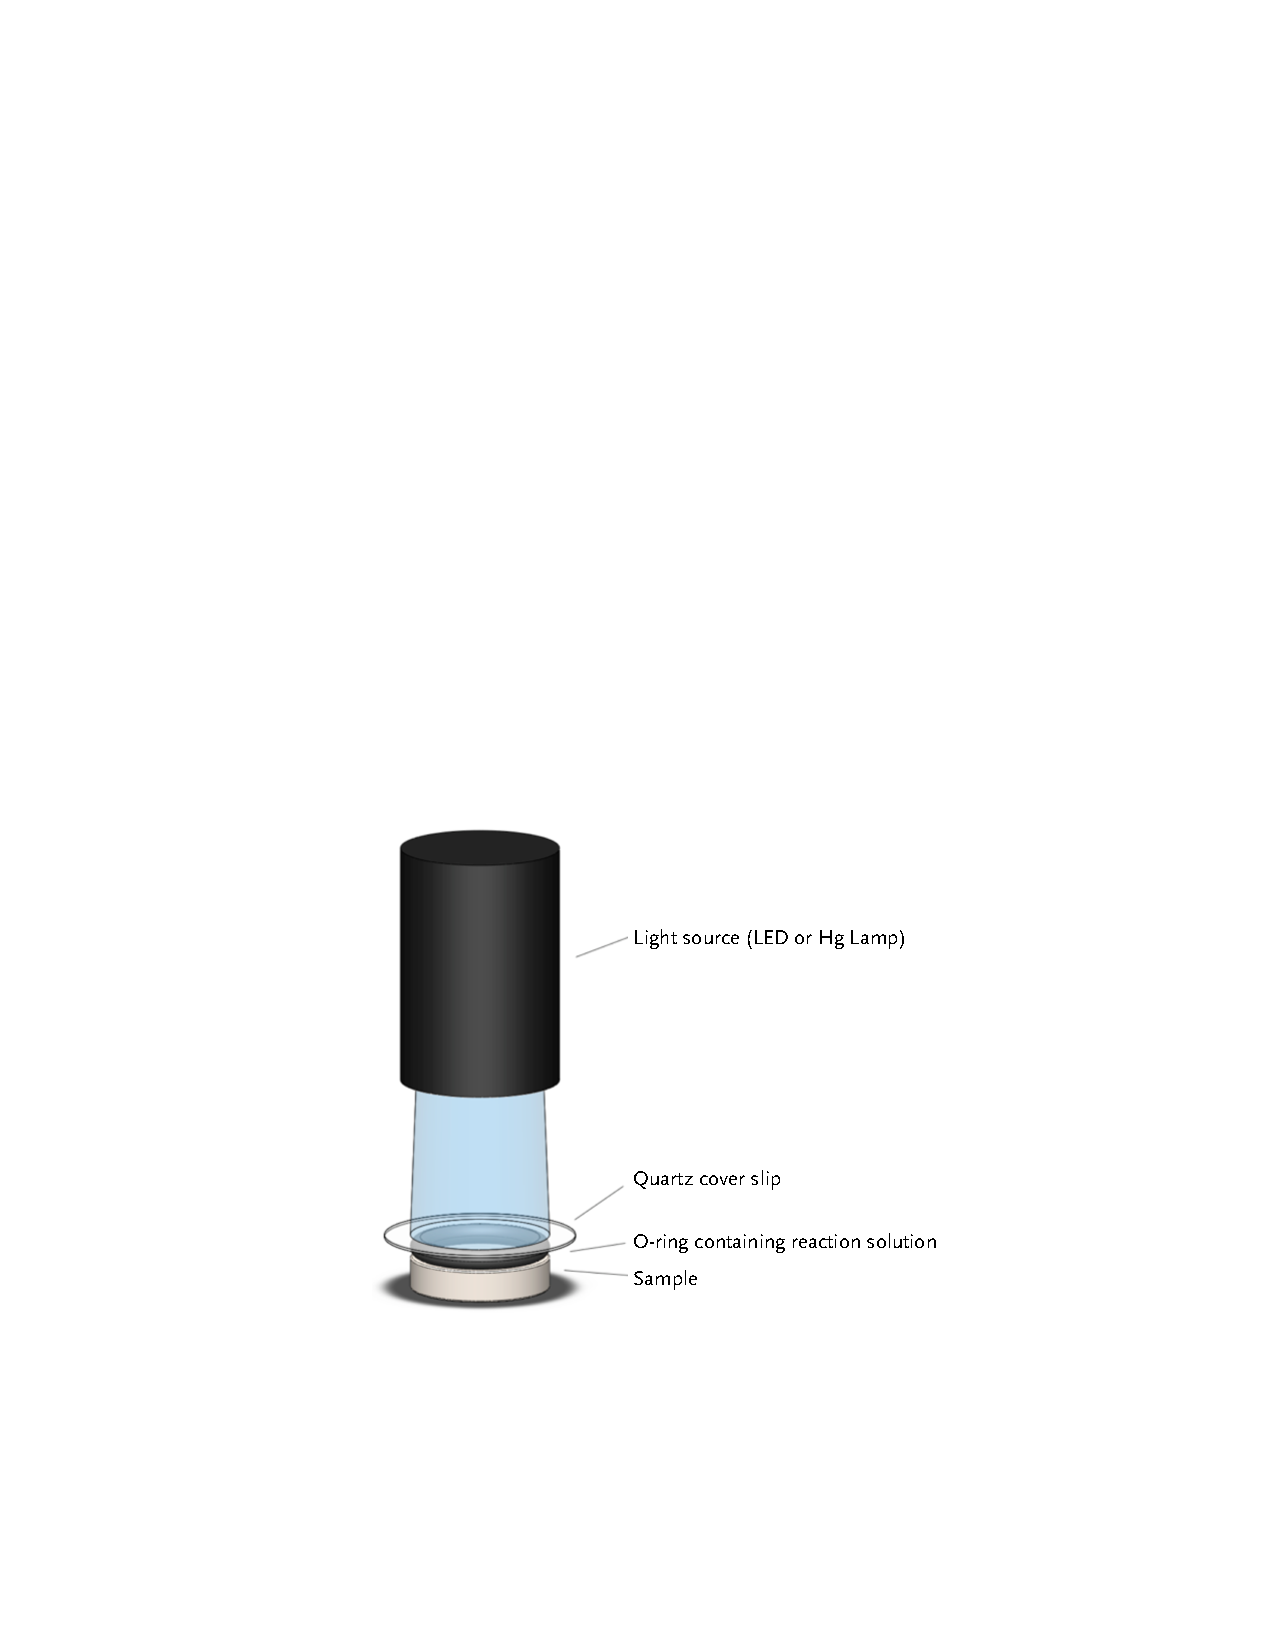
\includegraphics[width=\marginparwidth]{rxnsetup.pdf}
%}{0}
The established photochemical marker reaction of the reduction of silver ions in solution
to solid silver on the sample surface was used to study the photochemical reactivity of
the samples in this document.
\begin{equation}
\ce{Ag+ + e- -> Ag_{(s)}}
\end{equation}
This reaction deposits insoluble silver on the surface, marking the locations where
oxidation or reduction
occurred.\cite{Giocondi:2001gz,Burbure:2010go,Giocondi:2001bi,Burbure:2010ti,Bhardwaj:2010eh,%
Giocondi:2008ja,Lowekamp:1998ks,MorrisHotsenpiller:1998jq} The reaction product can
subsequently be observed using conventional atomic force microscopy methods.

For all marker reactions performed in this document, aqueous solutions of 0.115~\Molar
\ce{AgNO3} (Fisher Scientific, 99.96\%) were prepared. This specific concentration was
established by earlier
researchers,\cite{Giocondi:2001gz,Burbure:2010go,Giocondi:2001bi,Burbure:2010ti,Bhardwaj:2010eh,%
Giocondi:2008ja,Lowekamp:1998ks,MorrisHotsenpiller:1998jq} and results in an easily
observable reaction product on the surface after short illumination times.  Figure
\ref{fig:rxnsetup} schematically illustrates the setup for performing photochemical
reactions. A rubber O-ring was placed on the sample. A few drops of one of the solutions
were added into the O-ring. A quartz cover slip (\SI{0.2}{\milli\meter} thick) was placed
on top of the O-ring, held in place by surface tension. The cover slip creates a surface
perpendicular to the incident light, ensuring the same volume of solution and setup
geometry for all trials. The assembly was illuminated by commercially available blue
\abbr{LED} (\textlambda{}$_{\text{peak}}$ = \SI{470}{\nano\meter}, Philips Lumileds, San
Jose, CA) or \SI{300}{\watt} mercury arc lamp (Newport, Irvine, CA). The \abbr{LED} was
powered by a DC supply, set to deliver a constant current. Specific current and power
values for illumination are given along with corresponding experimental results in later
chapters. 

The duration of illumination varied, depending on the material and light source. The
reaction times used for collecting the data in this document were determined through
multiple trials, varying the reaction time in each trial. If the samples are allowed to
react for too long a duration, a the high amount of deposited solid makes characterization
difficult. Conversely, if the samples aren't reacted for a long enough time, the amount of
deposition is too low for observation. The times were selected because they resulted in an
observable and quantifiable amount of reaction product on the surface. Times for
individual photochemical experiments are listed in relevant sections of this document,
along with their corresponding results. After reaction, the samples were rinsed with
deionized water and dried with forced air.

To clean the surface of deposited products after reaction, the sample was wiped with a
cotton swab, then cleaned ultrasonically, first in methanol and then acetone. The acetone
was removed from the surface with a cotton swab. Subsequent microscopy demonstrates that
reaction products can be completely removed from the sample surface.

\label{masstransfer}
For all results presented in this document, it was assumed that mass transport of species
in the solution did not play a major role in interpreting the results from marker
reactions. The results from marker reactions presented in this document are all comparable
among experiments performed under the same conditions. For example,
\chapterref{single.crystal.reactivity} compares the relative reactivity of three
structures of \ce{Fe2O3} and \chapterref{fe2o3orientation} compares the relative
reactivity of different \ce{Fe2O3} grains on the same polycrystal. In these cases, certain
structures or grains were more reactive than others. It is possible that the rate of
reaction of the most reactive grains or structures was rapid enough that mass transfer
would be the limiting factor of reaction rate. However for each experiment, a comparison
between the most reactive and the least reactive structures could be made. Mass transfer
was not the limiting factor in the reactivity of the nonreactive or moderately reactive
cases, as under the same experimental conditions, other samples exhibited much higher
levels of reactivity.

\label{ph}
Reaction solution pH can potentially exert a significant effect on photochemical
properties of semiconductor photochemical systems. The pH of the solution affects the
nature of adsorbed species (typically, though not exclusively, \ce{H^{+}} and \ce{OH^{-}})
on the semiconductor surface, which in turn affect band bending within the space-charge
region of the semiconductor. The isoelectric point pH$_{\text{iep}}$ is defined as the pH
level at which the no net charge exists on the surface. A solution pH level higher than
this point causes a net negative charge on the surface, and a pH lower than the
pH$_{\text{iep}}$ causes a net positive charge on the surface. The effect of a solution pH
on the band edges of the semiconductor is given by
\begin{equation}
E_{CB}=E^{\degree}_{CB}+2.3kT\ln(\text{pH}-\text{pH}_{\text{iep}}),
\end{equation}
where $E{\degree}_{CB}$ is the band edge position at the isoelectric point. At room
temperature, this results in a band edge shift of \SI{60}{\milli\volt} with each
increasing pH unit. In the results presented in this document, pH effects are generally
not considered to have a major effect on the interpretation of activity results. The
reasoning for this is similar to that used for mass transfer effects.  In the case of
reactivity on \ce{Fe2O3} films, interpretations of results were comparative, with factors
affecting pH controlled across all experiments. As all films on single crystals were of
the same phase and orientation, negligible differences in pH effects between samples would
be expected. In the case of bulk \ce{Fe2O3} and \ce{Fe2O3} films on polycrystalline
substrates, in which the orientation of \ce{Fe2O3} is not controlled, differences in pH
could affect the reactivity of the individual film grains. The effect of surface
orientation on the isoelectric point varies depending on material. For example, the
isoelectric point of rutile \ce{TiO2} ranges between 3.2-3.7 for (100) faces and 5.5-5.8
for (001) faces,\cite{Bullard:2006jv} while the range of isoelectric points reported for
\textalpha-\ce{Fe2O3} is
6.3-8.5.\cite{Parks:1965ys,Kosmulski:2004vn,Kosmulski:2002kx,Kosmulski:2001ww} This
variance is somewhat significant, and can result in a band edge shift on the order of
\SI{100}{\milli\volt}. For the scope of the work presented in this document, that shift is
expected to be similar for all films, as preparation methods were consistent for all
samples, and reaction conditions were the same. 

\label{timescales}A last point to consider regarding the photochemical marker reactions
used in this work is differences in reactivity at various time scales. As the reaction
proceeds, the potential for changes in reaction conditions affecting reactivity exists.
The presence of silver on the surface immediately after the beginning of silver deposition
changes the overall band structure of the system. Early on in the reaction, most of the
surface is not covered by silver, but over longer timeframes, the affect of silver on the
band structure is no longer negligible. Once again, the comparative nature of the
interpretation of results should render negligible any affects from the change in the
electronic properties of the system from the deposition of silver. These effects would be
observed in all samples. Additionally, studies of the formation of silver nanoparticles in
aqueous solutions suggest that silver particles may grow
autocatalytically;\cite{Ershov:1993ci,VanHyning:2001vl} after the first silver atom forms,
additional silver atoms are easier to reduce and the rate of particle growth increases.
For the silver reaction product observed in the work presented in this document, distinct
silver particles are observed. Surfaces classified as more reactive in this work have more
individual particles on the surface. Thus the autocatalytic effects are not expected to be
responsible for the increased reactivity, as this would only expand already nucleated
particles.

\subsection{\abbr{EBSD}}
\label{subsec:exp.ebsd}


Electron backscatter diffraction (\abbr{EBSD}) was used as a primary tool for local
determination of film phase, orientation, and film|substrate orientation relationships.
Electron backscatter diffraction is a scanning electron microscopy technique that can
probe the local orientation and microstructure of a
material.\cite{Dingley:1997tw,Schwartz:2009ue} The technique relies on the interpretation
of an electron backscatter pattern. This pattern is generated when an electron beam
interacts with a flat surface, tilted at an angle of \texttildelow70\si{\degree}. The high
angle increases the intensity of backscattered electrons escaping from the sample.   As
backscattered electrons are generated in the electron beam interaction volume, they exit
the solid in patterns corresponding to the Bragg condition, a result of diffraction by
atomic planes within the material. The result is a  pattern of intersecting bands of high
intensity when the diffracted backscatter electrons reach a phosphor screen in the
\abbr{SEM} chamber. The phosphor screen is coupled to a \abbr{CCD} camera, which in turn
captures an image of the pattern. A schematic of this arrangement is depicted in Figure
\ref{fig:ebsdsetup}. 

\begin{figure}
\centering
	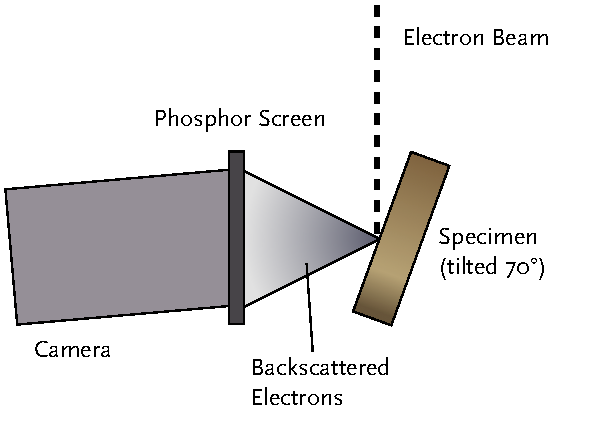
\includegraphics[width=0.8\textwidth]{ebsdsetup.pdf}
	\caption[Interior \abbr{SEM} arrangement for \abbr{EBSD} analysis]{%
	Schematic showing the interior arrangement of a scanning 
	electron microscope equipped with an \abbr{EBSD} detector.}
	\label{fig:ebsdsetup}
\end{figure}

\begin{figure}
\begin{center}
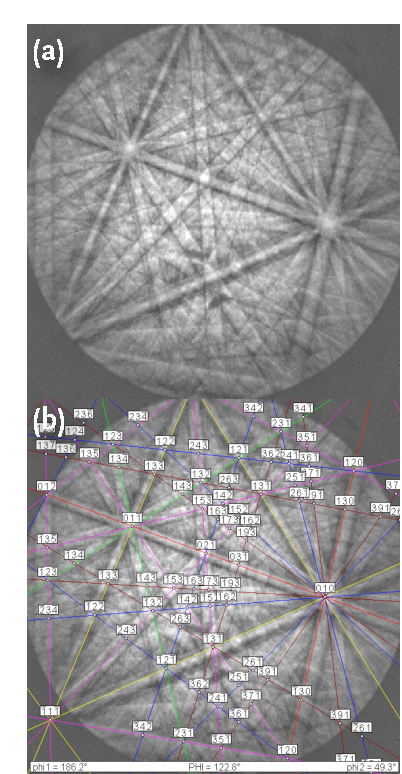
\includegraphics[width=0.4\textwidth]{ebsdsamples.pdf}
\caption[Electron backscatter diffraction patterns]{%
	Unindexed (a) and indexed (b) electron backscatter patterns 
	for a (111) oriented \ce{BiFeO3} grain.}
\label{fig:ebsdsamples}
\end{center}
\end{figure}
%\sidefigure[Electron backscatter diffraction patterns]{%
%	Unindexed (a) and indexed (b) electron backscatter patterns 
%	for a (111) oriented \ce{BiFeO3} grain.
%	\label{fig:ebsdsamples}
%	}{%
%	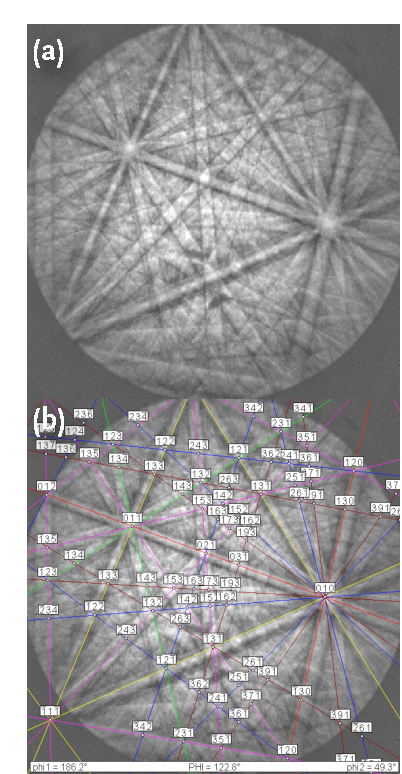
\includegraphics[width=\marginparwidth]{ebsdsamples.pdf}
%}{-21}
Computer software (\abbr{TSL}, \abbr{EDAX}, Mahwah, \abbr{NJ}), is used to then analyze
the location, intensity, and width of the bands. From this information, a set of Euler
angles is obtained that describes the orientation of the crystal. The Euler angles
represent the rotations that would rotate a crystal of a reference orientation to the
sample orientation. From the Euler angles, a set of Miller indices are generated
describing the local surface orientation in the crystal reference frame. A sample pattern
for a (111)-oriented \ce{BiFeO3} grain and the computer-generated band indexing is shown
in Figure \ref{fig:ebsdsamples}.


This procedure, if repeated across a raster pattern of points, can be used to map
orientations across a wide area of the sample. A computer can automate electron beam and
stage control, pattern acquisition, and pattern indexing. This technique has a benefit of
particular importance over other texture analysis techniques such as X-ray pole figures.
Orientation data is locally determined at each point, rather than over a wide area of the
sample simultaneously. This grants a great deal of flexibility when analyzing the
orientation data. Maps of grains, grain boundaries characterization, pole figures, and
inverse pole figures can be generated not just for the entirety  of the dataset, but also
for partitioned data of interest to a particular experiment. A representative map of grain
orientations for a \ce{SrTiO3} polycrystal is presented in Figure
\ref{fig:representativemap}.


\abbr{EBSD} was used in this work for analysis of \ce{Fe2O3} films grown on single crystal
and polycrystalline substrates. It was used for film phase identification, film
orientation measurement, and determination of epitaxial relationships between the film and
substrate. All electron backscatter experiments were performed in a Quanta 200
\abbr{FE-SEM} (\abbr{FEI} Company, Mahwah, \abbr{NJ}) equipped with and \abbr{EBSD}
detector using TSL software (\abbr{EDAX}) for pattern acquisition and data analysis.
\begin{figure}
\begin{center}
\includegraphics[width=0.75\textwidth]{representativemap.png}
\caption[Representative \abbr{EBSD} inverse pole map]{%
	Representative \abbr{EBSD} inverse pole map. This map depicts the 
	microstructure of a \ce{SrTiO3} polycrystal.}
\label{fig:representativemap}
\end{center}
\end{figure}
%\sidefigure[Representative \abbr{EBSD} inverse pole map]{%
%	Representative \abbr{EBSD} inverse pole map. This map depicts the 
%	microstructure of a \ce{SrTiO3} polycrystal.
%	\label{fig:representativemap}
%	}{%
%	\includegraphics[width=\marginparwidth]{representativemap.png}
%}{0}
All experiments were performed in a low-vacuum atmosphere in the presence of water vapor.
This allows for analysis of weakly conducting samples such as those used in this
experiment without the complications of sample charging from the electron beam. In all
cases, clearly indexable electron backscatter diffraction patterns were obtained, even
under low-vacuum conditions. The working distance was \SI{15}{\milli\meter}. The tilt
angle was always within \SI{0.1}{\degree} of of \SI{70}{\degree} from horizontal.
Accelerating voltage was 20.0-25.0~\si{\kilo\volt}. Exposure parameters for the \abbr{CCD}
camera were adjusted as needed for each scan. Generally, the exposure time was adjusted to
achieve a frame rate of 50-100~frames~per~second. Other parameters were then adjusted to
obtain diffraction patterns with good contrast and accurate indexing of diffraction bands,
as determined by manual inspection and computer-generated confidence index (\abbr{CI}). 
Computer image processing was used to improve the pattern quality. An average background
signal was collected while scanning the beam over the sample. This background is
subtracted by the computer for all collected patterns, to increase the contrast of the
pattern. In some cases, additional processing such as dynamic background subtraction and
normalizing of the intensity histogram were required to obtain good patterns. Scan
parameters such as the scan area and distance between points were changed from sample to
sample, and were dependent upon grain size, frame rate, and available microscope time.


\subsection{X-ray}
\label{subsec:exp.xray}


Conventional X-ray diffraction (\abbr{XRD}) characterization was used to verify the phase
of polycrystalline samples and to determine the phase and orientation of thin film
samples. In the experiments presented in this document, X-ray diffraction was used to
verify the presence of a desired phase in synthesized materials. X-ray scans were
performed using a Panalytical X'Pert Pro \abbr{MPD} diffractometer (Panalytical,
Westborough, \abbr{MA}). After the diffraction pattern was collected, the results were
compared with tabulated diffraction data from the International Center for Diffraction
Data database. 

X-ray reflectometry\cite{birkholz2006thin} was used to measure film thickness and
calibrate growth rate. X-ray reflectivity relies upon interference between reflected beams
from layers of material with different density. In this technique, the incident angle of
the X-ray beam is slowly varied. As the reflected angle is changed, interaction between
the reflected beam switches between constructive and destructive interference, causing
fringes in the collected intensity data. Software is then used to calculate film
thickness, given information about the composition and density of the materials under
investigation. X-ray reflectometry scans were carried out on a Panalytical diffractometer.
Using this data, the growth rate for films under the deposition conditions used in this
document was determined. This growth rate was then used to select the appropriate
deposition duration to deposit films of desired thicknesses. 


\subsection{Scanning Probe Microscopy}
\label{subsec:exp.scanningprobe}


Sample surface profiles before and after photochemical reaction were examined using
contact mode atomic force microscopy (\abbr{AFM}). \abbr{AFM} determines nanoscale
displacements by measuring the deflection of a laser beam reflected off a microscopic
cantilever.\cite{Murphy:1987wc} Attached to the cantilever is a tip that moves along the
surface of the sample. Piezoelectric elements are used to scan the tip across the sample.
As the height of the sample changes, the tip is deflected, changing the measured intensity
of the reflected beam. The microscope adjusts the height of the tip to account for the
deflection, recording the magnitude of the adjustment. The records for the entire scanned
area are constructed into an image corresponding to the topography of the sample. 

\abbr{AFM} micrographs of sample surfaces were recorded before and after photochemical
marker reactions. Conventional contact and semicontact methods were
used.\cite{Anonymous:YBI-TQ6H} All scans were collected on either an \abbr{NT}egra or
Solver Next \abbr{AFM} (\abbr{NT-MDT}, Moscow, Russia). For contact mode images, aluminum
coated silicon tips with a force constant of 0.11~\si{\newton\per\meter} were used
(\abbr{CSG10, NT-MDT}). For semicontact images, aluminum coated silicon tips with a rated
resonant frequency of 240~\si{\hertz} were used (\abbr{NSG10, NT-MDT}). Scan rates were
chosen based on the size of the scan area, and were in the range of 0.5-2~\si{\hertz}.  

The local surface polarization of \ce{BiFeO3} was examined using piezoresponse force
microscopy (\abbr{PFM}). Piezoresponse force is a contact mode technique used to determine
the local polarization direction of ferroelectric
materials.\cite{Kalinin:2002hq,Kalinin:2006bg,Jungk:2006he,Rodriguez:2004bu} While
scanning the surface in contact mode, an \abbr{AC} bias is applied to the tip. Because
ferroelectric materials are also piezoelectric, the applied bias causes a local expansion
or contraction of the material. A lock-in amplifier is used to measure the phase of the
expansion and contraction. From this data, the out of plane direction of polarization of
the surface is determined. \abbr{PFM} measurements were collected using a
Solver\abbr{NEXT} \abbr{AFM}. Titanium nitride coated tips with a force constant of
11.8~\si{\newton\per\meter} were used (\abbr{NSG10}/Au, \abbr{NT-MDT}).